\documentclass[a4paper,10pt]{article}
\usepackage[utf8]{inputenc}

%pour les equations
\usepackage{amsmath}
\usepackage{amssymb}
\usepackage{amsfonts}

%pour les images
\usepackage{graphicx}

% pour definir des couleurs
\usepackage{xcolor}

% pour inclure du code
\usepackage{listings}

\usepackage{csquotes}

% code color
\definecolor{ligthyellow}{RGB}{250,247,220}
\definecolor{darkblue}{RGB}{5,10,85}
\definecolor{ligthblue}{RGB}{1,147,128}
\definecolor{darkgreen}{RGB}{8,120,51}
\definecolor{darkred}{RGB}{160,0,0}

\lstset{
    language=C++,
    captionpos=b,
    extendedchars=true,
    frame=lines,
    numbers=left,
    numberstyle=\tiny,
    numbersep=5pt,
    keepspaces=true,
    breaklines=true,
    showspaces=false,
    showstringspaces=false,
    breakatwhitespace=false,
    stepnumber=1,
    showtabs=false,
    tabsize=3,
    basicstyle=\small\ttfamily,
    backgroundcolor=\color{ligthyellow},
    keywordstyle=\color{ligthblue},
    morekeywords={include, printf, uchar},
    identifierstyle=\color{darkblue},
    commentstyle=\color{darkgreen},
    stringstyle=\color{darkred},
}

%opening
\title{Image Couleur}
\author{Elliot Vanegue}

\begin{document}

\maketitle
\section{Introduction}
\paragraph{}Le but de ce TP est d'observer l'impacte de la luminance et de la saturation sur les informations
contenues dans une image. Pour cela, nous allons travailler avec ImageJ et deux plug in fourni pour
ce TP.

\section{Manipulation luminance}
\paragraph{}Nous allons dans un premier comparer deux images \textit{it1\_72pp} et \textit{it1\_72pp\_sombre}, la seconde étant plus sombre que l'autre.
La clarté d'une image dépend de l'information de luminance.
Pour effectuer cette comparaison, nous allons devoir utiliser un autre espace colorimètrique qui
sait représenter cette information. Plusieurs espaces sont disponible comme le YUV ou le HSV.
Dans notre cas, nous allons prendre l'espace HSV dont la valeur (\enquote{value}) représente 
la luminance présente dans l'image.\\

\begin{figure}[!h]
 \begin{center}
 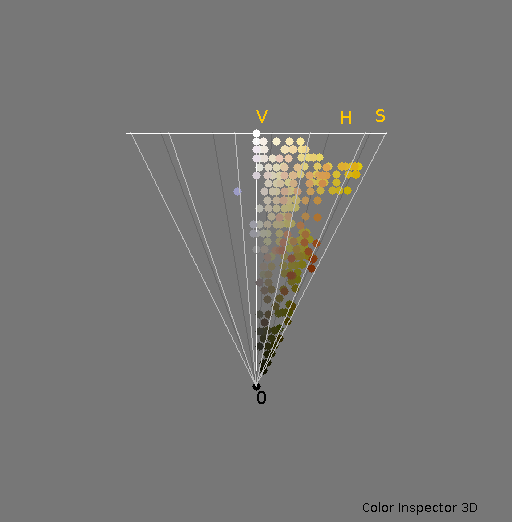
\includegraphics[width=4cm]{resultat/luminance1.png}
 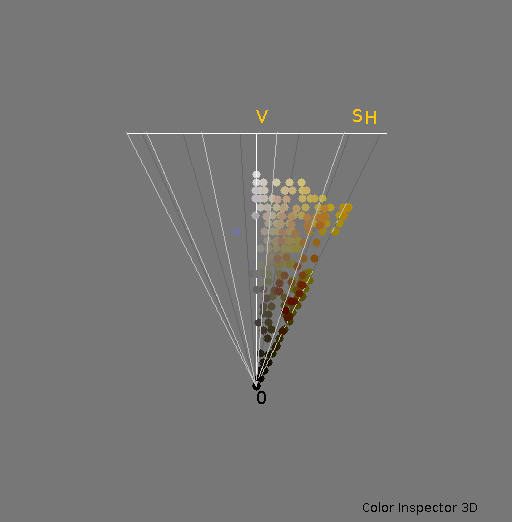
\includegraphics[width=4cm]{resultat/luminance2.png}
 \caption{Graphique de l'espace colorimétrique HSV des images \textit{it1\_72pp} et \textit{it1\_72pp\_sombre}}
 \end{center}
\end{figure}

On voit clairement que la plus grande valeur de luminance de l'image sombre est bien inférieur
à la valeur maximum de l'image plus claire. En effet, l'image qui est plus sombre ne possède pas de pixel dans le haut du conne
HSV.\\

Nous allons maintenant essayer de transformer l'image la plus sombre en l'image originale. Pour cela,
nous allons simplement ajouter une valeur identique dans les trois canaux RGB. Etant donné que la valeur 255
représente le blanc, il est possible d'éclaircir l'image en rapprochant la valeur de chaque canaux de la valeur 255.

%TODO affichage des résultats de chaque image
\begin{tabular}{|c|c|c|}
 
\end{tabular}

%TODO question 4 a voir

\section{Rétablissement de la saturation}
La saturation peut-être défini comme étant la chromaticité de la couleur. Elle est l'intensité de la couleur, plus
la saturation est faible et plus la couleur paraît fade. Pour mettre en évidence cette saturation, nous analysons
l'espace colorimètrique HSV des images \textit{it2\_72pp} et \textit{it2\_72\_gris}, dont la première est plus saturé
que la seconde.\\

\begin{figure}[!h]
 \begin{center}
 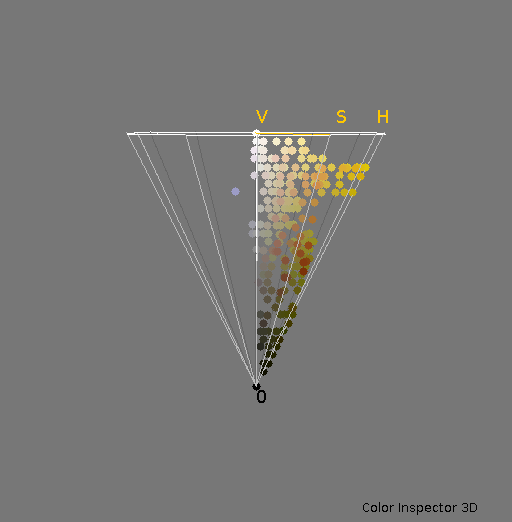
\includegraphics[width=4cm]{resultat/saturation1.png}
 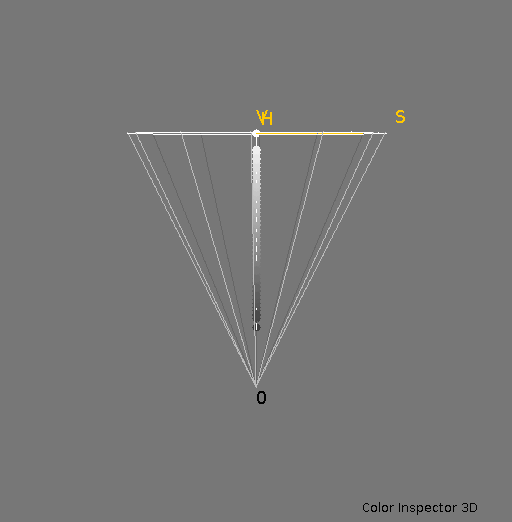
\includegraphics[width=4cm]{resultat/saturation2.png}
 \caption{Graphique de l'espace colorimétrique HSV des images \textit{it2\_72pp} et \textit{it2\_72\_gris}}
 \end{center}
\end{figure}

Sur ces images, l'information de saturation est représenté sur l'axe des x. On voit que sur l'image \textit{it2\_72\_gris} la
valeur de la saturation reste à 0, ce qui fait que l'ensemble des pixels restent au centre du conne. On voit qu'il n'est pas
possible de transformer l'image \textit{it2\_72\_gris} en l'image \textit{it2\_72pp}, car l'information \textit{value} n'est pas
connu et l'image ne changerai pas si on modifiait la saturation. C'est pourquoi nous utiliserons l'image \textit{it2\_72\_saturation\_faible}
pour nos test sur le changement de la saturation. Voici dans un premier temps les graphiques des image dans le modèle HSB.

\begin{figure}[!h]
 \begin{center}
 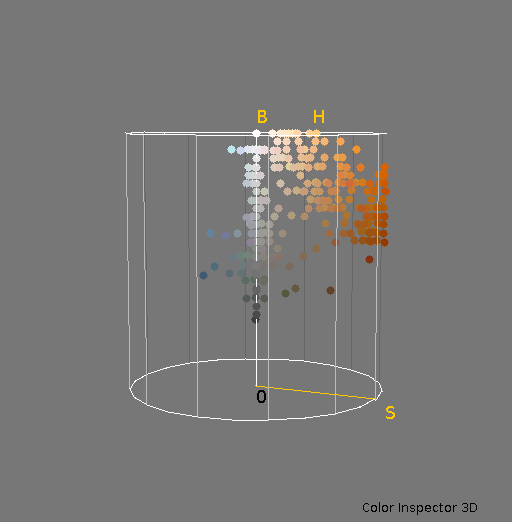
\includegraphics[width=4cm]{resultat/saturation1_2.png}
 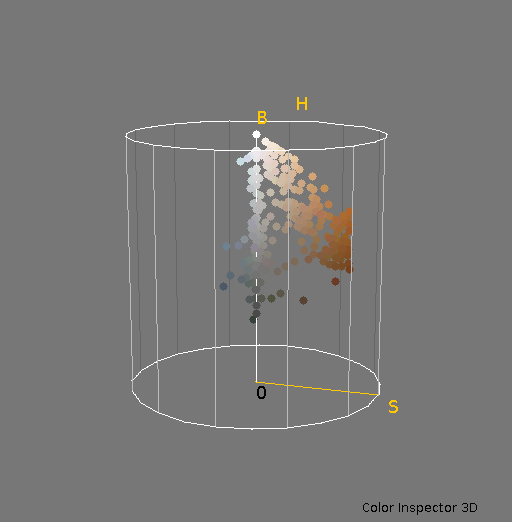
\includegraphics[width=4cm]{resultat/saturation2_2.png}
 \caption{Graphique de l'espace colorimétrique HSB des images \textit{it2\_72pp} et \textit{it2\_72\_saturation\_faible}}
 \end{center}
\end{figure}
\newpage

On voit avec ces graphique que l'image \textit{it2\_72\_saturation\_faible} possède un \textit{value} différent de 0, donc si on 
multiplie la saturation par une valeur défini il est possible de retrouver l'image \textit{it2\_72pp}. Cependant, on voit que 
la saturation n'est pas la seul valeur qui différencie les deux images, la luminance est également très différente. En multipliant
la saturation par 1,3 nous obtenons le résultats suivant :

\begin{figure}[!h]
 \begin{center}
 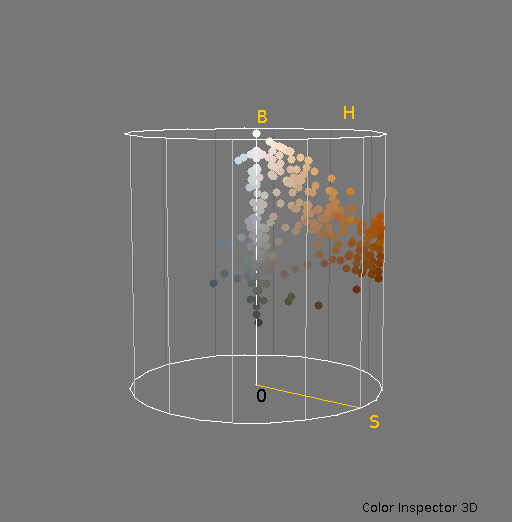
\includegraphics[width=4cm]{resultat/resultat_saturation.png}
 \caption{Résultat de la modification de la saturation}
 \end{center}
\end{figure}

\section{Transformation de la teinte}
La teinte est la forme la plus pure d'une couleur. Ce qui signifie qu'elle ne peut pas représenté le blanc, le noire ou le gris.
Pour modifier la couleur de l'image pour que le chiffre devienne vert, nous modifions la teinte en lui ajoutant la valeur 90.
Nous avons pris la valeur 90, car on peut voir que sur le cercle de la teinte que le vert est a peu près a 90° de la couleur bleu.
Cela nous donne le résultat suivant : 
\begin{figure}[!h]
 \begin{center}
 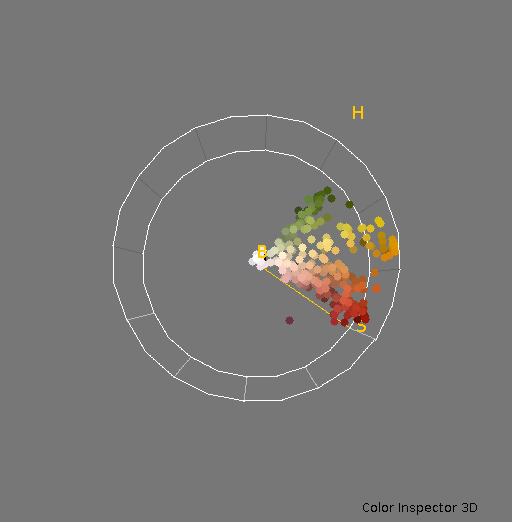
\includegraphics[width=4cm]{resultat/teinte1.png}
 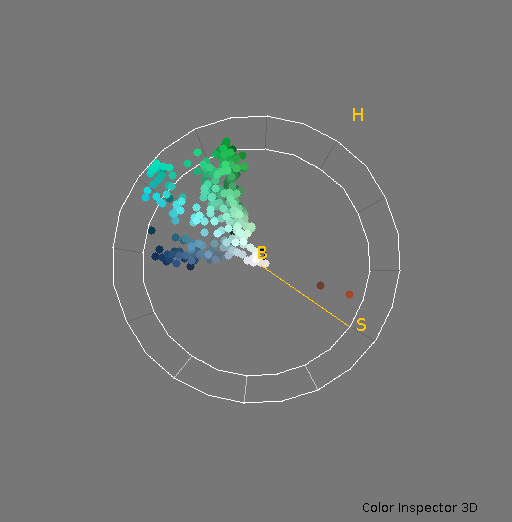
\includegraphics[width=4cm]{resultat/teinte2.png}
 \caption{Graphique de l'espace colorimétrique HSB de l'images \textit{it3_72pp} et du résultat de la transformation}
 \end{center}
\end{figure}

\end{document}
